\documentclass{standalone}
\usepackage{tikz}
\usetikzlibrary{arrows}
\begin{document}
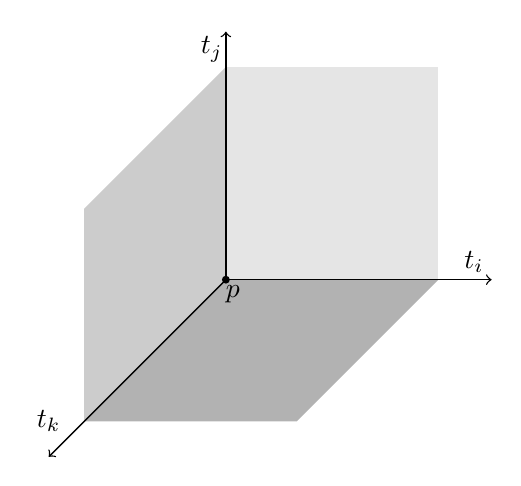
\begin{tikzpicture}[scale=(0.45),arrow/.style={->, >=angle 90}]
\fill[black!20!] (-4,-4) -- (-4,2) -- (0,6) -- (0,0) -- cycle;
\fill[black!10!] (0,6) -- (6,6) -- (6,0) -- (0,0) -- cycle;
\fill[black!30!] (-4,-4) -- (2,-4) -- (6,0) -- (0,0) -- cycle;
\draw [->,line width=.5pt] (0,0) -- (7.5,0);
\draw [->,line width=.5pt] (0,0) -- (0,7);
\draw [->,line width=.5pt] (0,0) -- (-5,-5);

% ORIENTATION ARROWS ON FACES
%\def\barrow at (#1,#2) {
%	\draw [line width=.8pt, black!70!] (#1,#2) ++(140:5mm) arc (-220:40:7mm);
%	\draw [line width=.8pt, black!70!] (#1+.7,#2+.3) -- (#1+.65,#2-.1);
%	\draw [line width=.8pt, black!70!] (#1+.7,#2+.3) -- (#1+1.05,#2+.1);
%}
%
%	\barrow at (2.9,3.2)
%\begin{scope}[cm={1,0,.5,.8,(0,0)}]
%	\barrow at (2,-2.5)
%\end{scope}
%\begin{scope}[cm={.9,.7,0,.9,(0,0)}]
%	\barrow at (-2.2,2.8)
%\end{scope}

% ORIENTATION ARROWS ON EDGES & EDGE LABELS
%\draw [->,line width=.5pt] (2,.3) -- (4,.3);
%\node at (3,-.5) {$\partial S_i$};
%
%\draw [->,line width=.5pt] (-.3,2) -- (-.3,4);
%\node at (.7,3) {$\partial S_j$};
%
%\draw [->,line width=.5pt] (-1,-1.5) -- (-2.5,-3);
%\node at (-2.5,-1.5) {$\partial S_k$};

\node [circle, fill=black,inner sep=0, minimum size=1mm] at (0,0) {};
\node at (.2,-.4) {$p$};
\node at (7,.5) {$t_i$};
\node at (-.4,6.5) {$t_j$};
\node at (-5,-4) {$t_k$};
%\node at (5,5) {$S_{ij}$};
%\node at (-3.1,1.6) {$S_{jk}$};
%\node at (1.5,-3.3) {$S_{ki}$};
\end{tikzpicture}
\end{document}